\tikzset{%
  % Specifications for style of nodes:
         base/.style =  { rectangle, rounded corners, draw = black, minimum width=2.5cm, minimum height=1cm, font=\ttfamily },
         node/.style =  { base, fill=orange!15 },
         begin/.style = { base, fill=blue!30 },
         end/.style =   { base, fill=red!30 },
}

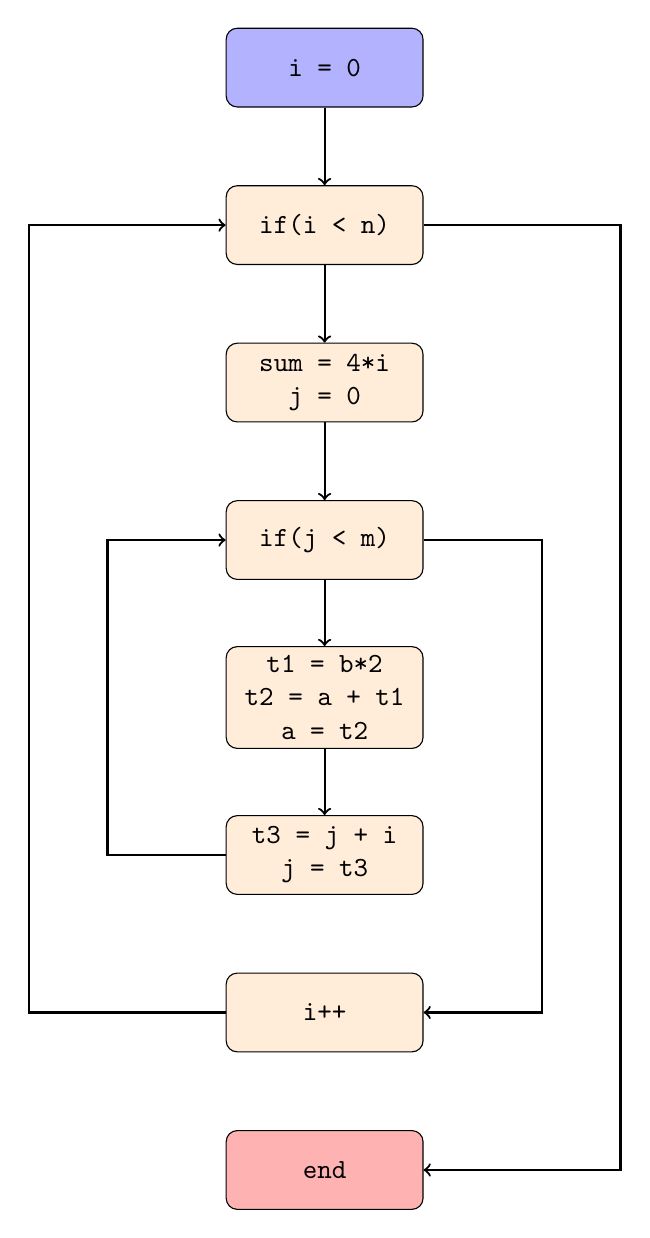
\begin{tikzpicture}[node distance=2cm, every node/.style={fill=white, font=\sffamily}, align=center]
    % Draw nodes
    \node (start)       [begin]                        {i = 0};
    \node (if_1)        [node, below of = start]       {if(i < n)};
    \node (block)       [node, below of = if_1]        {sum = 4*i \\ j = 0};
    \node (if_2)        [node, below of = block]       {if(j < m)};
    \node (block_2)     [node, below of = if_2]        {t1 = b*2 \\ t2 = a + t1 \\ a = t2};
    \node (block_3)     [node, below of = block_2]     {t3 = j + i \\ j = t3};
    \node (block_4)     [node, below of = block_3]     {i++};
    \node (end)         [end, below of = block_4]      {end};

    % Draw arrows
    \draw[->,thick]           (start) -- (if_1);
    \draw[->,thick]           (if_1) -- (block);
    \draw[->,thick]           (block) -- (if_2);
    \draw[->,thick]           (if_2) -- (block_2);
    \draw[->,thick]           (block_2) -- (block_3);

    \draw[->,thick]           (block_3.west) -- ++(-1.5,0) -- ++(0,4) -- ++(1.5,0) (if_2);
    \draw[->,thick]           (if_2.east) -- ++(1.5,0) -- ++(0,-6) -- ++(-1.5,0) (block_3);
    \draw[->,thick]           (block_4.west) -- ++(-2.5,0) -- ++(0,10) -- ++(2.5,0) (if_1);
    \draw[->,thick]           (if_1.east) -- ++(2.5,0) -- ++(0,-12) -- ++(-2.5,0) (end);
\end{tikzpicture}
